% docs/Latex/ClaftaxResult.tex -- working note (not a formal paper): Phase-1 model families on Craftax-Classic.
% Source of every number: output/phase1/ (per-seed JSON), aggregated by scripts/aggregate_phase1.py.
% Full write-up: docs/experiments/2026-09-30_phase1_model_families/README.md ; STATE task TASK-20260930-017.
\documentclass[10pt]{article}
\usepackage[margin=2cm]{geometry}
\usepackage{booktabs,graphicx,array,xcolor,hyperref,amsmath,parskip}
\graphicspath{{figures/}}
\newcommand{\p}[1]{\texttt{\small #1}}
\setlength{\tabcolsep}{4pt}
\title{Phase-1 model families on Craftax-Classic:\\ pure RL vs Transformer vs world-model features vs ChunkPPO}
\author{Run 2026-09-30/10-01, local RTX 3060 Ti; branch \p{claude/reasoning-model-baselines-38c2e9}}
\date{}
\begin{document}
\maketitle

% ERRATUM added 2026-10-04 (audit TASK-20261004-022); ClaftaxResult.pdf predates it and was not rebuilt.
\noindent\fbox{\parbox{\dimexpr\linewidth-2\fboxsep}{\small\textbf{Erratum (2026-10-04, audit TASK-20261004-022).} The \p{tf\_gru} win below
($39.2\pm1.3$, $\Delta=+5.6\pm1.5$) is \textbf{not reliable and must not be cited}: its learning rate was selected with runs produced by
uncommitted code (recorded commit cb35899 has no \p{tf\_gru} arm), it was designed after seeing the other arms on the same evaluation seeds,
and it did not replicate (TASK-020: $34.19\pm1.62$ on fresh seeds 42--51, $+1.7$ vs \p{ppo\_gru}, n.s.; same-seed reruns of its tuning
runs 34.1/34.0 instead of 41.4/43.1). No number was fabricated; the other conclusions stand.
See \p{docs/experiments/2026-10-04\_phase1\_score\_audit/README.md}.}}

\section*{Summary}
\begin{itemize}\itemsep0pt
\item \textbf{None of the four requested families beat pure RL} (100k and 1M steps): pure Transformer, Transformer + Idea-6 world-model (WM) features, ChunkPPO ($k{=}1$).
\item \textbf{Trained WM features = frozen random WM}: reward\_pct $-0.05\pm0.36$ (100k), $+1.4\pm1.2$ (1M); both n.s.
\item \textbf{One derivative model wins at 1M:} \p{tf\_gru} = tile-token Transformer encoder + GRU memory (PPO, 0.45M params): $39.2\pm1.3$ / $11.5\pm0.5$ vs best pure RL (GRU) $33.6\pm0.8$ / $9.1\pm0.5$, $\Delta=+5.6\pm1.5$ / $+2.3\pm0.7$. Neither part alone does it (Transformer without memory 29.2; GRU without Transformer 33.6; CNN+GRU control 33.0). No WM, search or chunking involved. Designed \emph{after} seeing the other 1M results; passed one clean test on 10 fresh seeds.
\item \textbf{No roadmap gate claimed.} G1.0 fails: best baseline 33.6/9.1 vs required $\ge 42.7/\ge 9.6$ ($0.9\times$ MFRL\_4M\_reimpl, Dedieu 2025 Table 1), so Phase-1 comparisons are internal only. \p{tf\_gru} reward $39.2<47.40$; score $11.45-2\cdot0.45=10.55<10.71$.
\item 100k runs (requested budget) show no separation between architectures. The 1M runs are a deliberate extension (cost 5--60 min/seed locally; only they can speak to the gates). Nothing above 1M was run.
\end{itemize}

\section*{Setup}
\textbf{Env/obs:} \p{CraftaxClassicSymbolicEnv}, default params (limit 10\,000 steps, no T cap), raw 1345-d symbolic obs ($7{\times}9{\times}21$ tiles + 22 scalars), 17 actions, unchanged reward.
\textbf{Protocol:} \emph{EP-A-mini} ($\le$100k steps, 98\,304--99\,840 executed; never gating) and \emph{EP-A} (999\,424 steps, 10 seeds 0--9). Sampled policy, first episode of 256 fresh envs/seed, final params; tuning seeds $\ge$1000 (disjoint), same grid for every arm (100k: n16$\times$T32 / n64$\times$T64 $\times$ lr\{3e-4,1e-3,3e-3\}, 3 seeds; 1M: lr\{3e-4,1e-3,3e-3\} at n64$\times$T64, 2 seeds). Selection = mean reward\_pct on tuning seeds.
\textbf{Metrics} (\emph{metric\_check} done by code reading + unit tests): reward\_pct = mean (distinct achievements/22)$\times$100 via \p{masked\_achievements()}; score\_pct = $\exp(\frac1{22}\sum_i\ln(1+s_i))-1$. Untrained init policy: $10.17\pm0.15$ / $1.75\pm0.03$.

\begin{table}[h]\centering\small
\begin{tabular}{@{}p{2.3cm}p{8.4cm}rr@{}}\toprule
arm & description & params\_total & deployed\\\midrule
\p{ppo\_mlp} & PPO, two tanh MLPs $3{\times}512$ (pure RL) & 2.44M & 1.22M\\
\p{ppo\_gru} & embed $\to$ GRU(256) $\to$ heads (pure RL, recurrent) & 0.88M & 0.81M\\
\p{tf} & Transformer d64/2L over 63 tiles + scalars + 4 history steps + 17 candidate-action tokens + CLS; logits from candidate tokens & 0.20M & 0.20M\\
\p{tf\_wm} & \p{tf} + action-conditioned 1-step WM features per candidate action (no noop future; trained only on the executed transition; stop-grad) & 0.98M & 0.98M\\
\p{tf\_wm\_random} & control: same, WM frozen at random init & 0.98M & 0.98M\\
\p{chunkppo\_k1} & \p{chunk\_ppo.py}, chunk Transformer actor over [state, 4 hist], MLP critic, $k{=}1$ & 1.41M & 0.19M\\
\emph{\p{tf\_gru}} & per-step \p{tf} encoder (no history tokens) $\to$ GRU(256) & 0.45M & 0.45M\\
\emph{\p{cnn\_gru}} & control: 2-layer CNN encoder $\to$ same GRU & 1.59M & 1.53M\\\bottomrule
\end{tabular}
\caption*{Italic = derivative arms added after the main comparison.}
\end{table}

\section*{Results}
Mean $\pm$ SE over 10 seeds; $\Delta$ = difference to the reference arm $\pm$ Welch SE. Per-seed values: \p{output/phase1/final\_*\_all/}.

\begin{table}[h]\centering\small
\begin{tabular}{@{}lrrrr@{}}\toprule
\multicolumn{5}{c}{\textbf{$\le$100k steps (EP-A-mini)}, reference = \p{ppo\_mlp}}\\
arm & reward\_pct & score\_pct & $\Delta$reward & $\Delta$score\\\midrule
\p{ppo\_mlp}   & $20.10\pm0.16$ & $3.71\pm0.09$ & -- & --\\
\p{ppo\_gru}   & $20.06\pm0.28$ & $3.16\pm0.10$ & $-0.03\pm0.32$ & $-0.56\pm0.14$\\
\p{cnn\_gru}   & $18.97\pm0.28$ & $3.00\pm0.09$ & $-1.13\pm0.33$ & $-0.71\pm0.13$\\
\p{chunkppo\_k1} & $18.60\pm0.33$ & $3.03\pm0.12$ & $-1.50\pm0.36$ & $-0.68\pm0.16$\\
\p{tf}         & $18.17\pm0.28$ & $3.31\pm0.07$ & $-1.92\pm0.32$ & $-0.41\pm0.12$\\
\p{tf\_gru}    & $17.94\pm0.16$ & $3.33\pm0.09$ & $-2.15\pm0.23$ & $-0.38\pm0.13$\\
\p{tf\_wm\_random} & $17.69\pm0.31$ & $2.92\pm0.08$ & $-2.40\pm0.35$ & $-0.80\pm0.13$\\
\p{tf\_wm}     & $17.64\pm0.18$ & $3.07\pm0.06$ & $-2.46\pm0.24$ & $-0.65\pm0.11$\\\bottomrule
\end{tabular}
\caption*{Derivative arms use the config selected at 1M (no 100k tuning). 100k is too little for any architecture to leave the starter achievements (nothing reaches stone).}
\end{table}

\begin{table}[h]\centering\small
\begin{tabular}{@{}lrrrr@{}}\toprule
\multicolumn{5}{c}{\textbf{1M steps (EP-A protocol)}, reference = \p{ppo\_gru}}\\
arm & reward\_pct & score\_pct & $\Delta$reward & $\Delta$score\\\midrule
\p{tf\_gru}    & $\mathbf{39.19\pm1.27}$ & $\mathbf{11.45\pm0.45}$ & $+5.61\pm1.52$ & $+2.33\pm0.66$\\
\p{ppo\_gru}   & $33.57\pm0.83$ & $9.12\pm0.48$ & -- & --\\
\p{cnn\_gru}   & $32.95\pm0.57$ & $8.35\pm0.40$ & $-0.63\pm1.00$ & $-0.77\pm0.63$\\
\p{ppo\_mlp}   & $30.14\pm0.46$ & $7.08\pm0.36$ & $-3.43\pm0.95$ & $-2.04\pm0.60$\\
\p{tf}         & $29.24\pm0.36$ & $6.67\pm0.31$ & $-4.34\pm0.91$ & $-2.46\pm0.57$\\
\p{tf\_wm}     & $28.58\pm0.75$ & $6.71\pm0.47$ & $-5.00\pm1.12$ & $-2.41\pm0.67$\\
\p{tf\_wm\_random} & $27.16\pm0.93$ & $5.86\pm0.51$ & $-6.42\pm1.25$ & $-3.26\pm0.71$\\
\p{chunkppo\_k1} & $23.90\pm0.34$ & $4.58\pm0.12$ & $-9.68\pm0.90$ & $-4.54\pm0.50$\\\bottomrule
\end{tabular}
\caption*{Selected lr: 1e-3 for all except \p{tf\_wm} (3e-3) and \p{chunkppo\_k1} (3e-4); all n64$\times$T64. \p{tf\_gru} tuning lr: 3e-4 $\to$ 27.3, 1e-3 $\to$ 42.3, 3e-3 $\to$ 30.0 (1 seed). Episodes are short for every arm (mean 140--230 steps, none censored), so these are early-game results.}
\end{table}

\begin{figure}[h]\centering
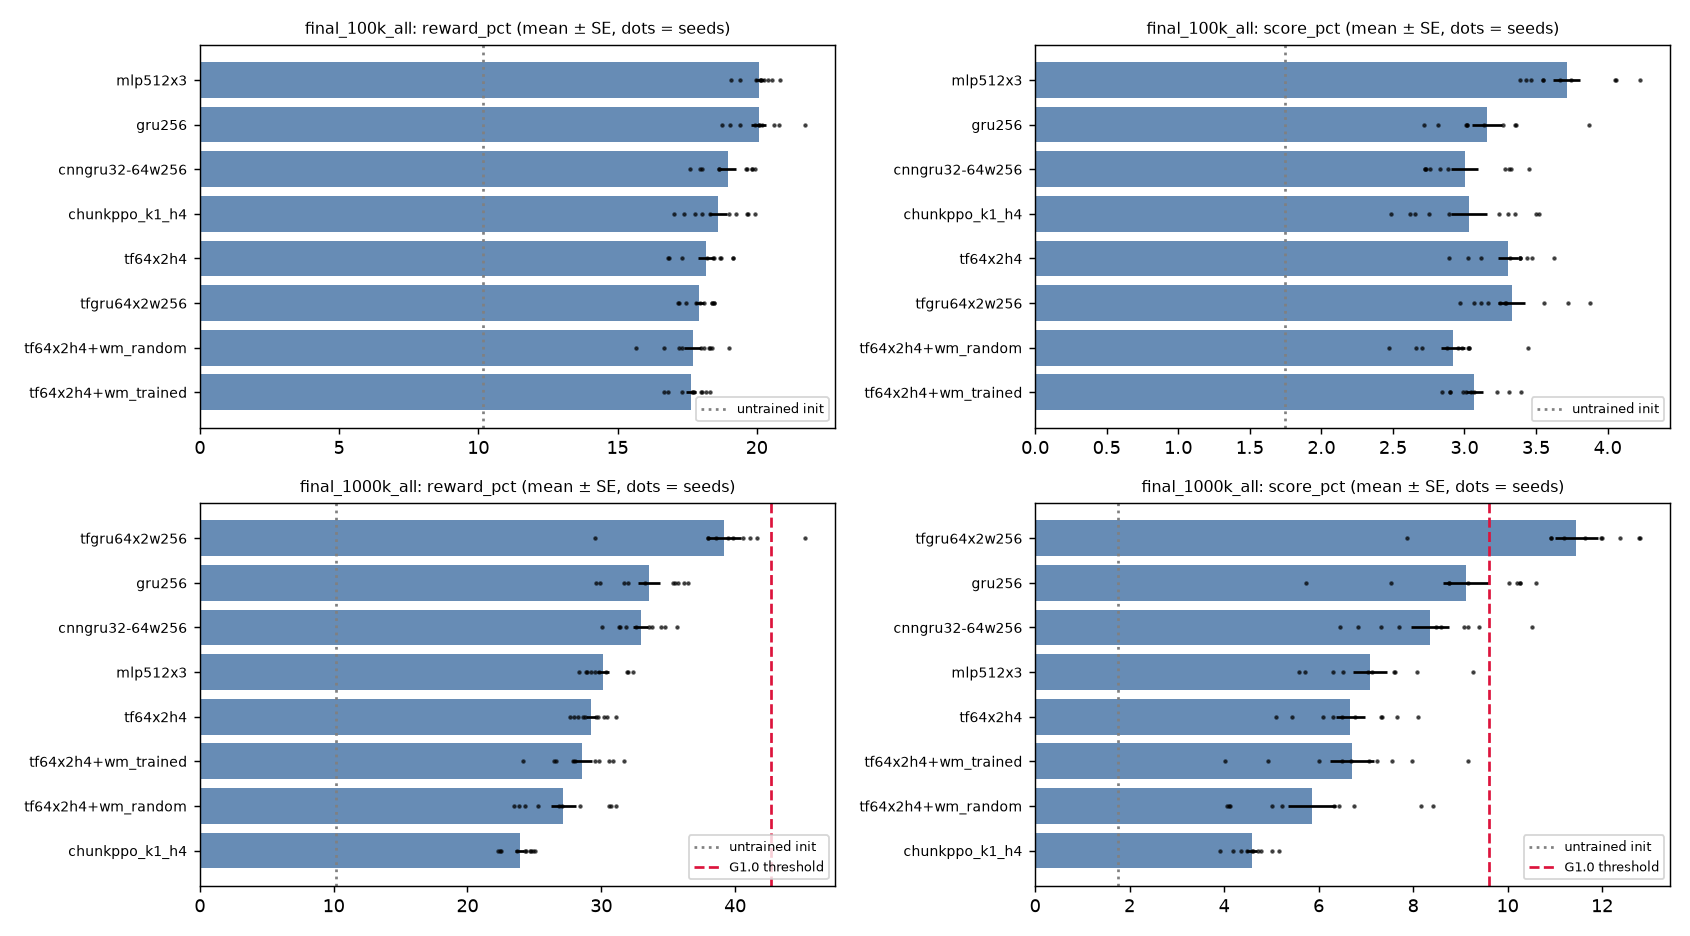
\includegraphics[width=\textwidth]{phase1_results.png}
\caption{reward\_pct and score\_pct per arm (bars = mean $\pm$ SE, dots = seeds). Top: $\le$100k; bottom: 1M with the G1.0 thresholds (red dashed) and the untrained policy (grey dotted).}
\end{figure}

\begin{table}[h]\centering\footnotesize
\begin{tabular}{@{}lrrrrrrrr@{}}\toprule
unlock \% (1M) & \p{tf\_gru} & \p{gru} & \p{cnn\_gru} & \p{mlp} & \p{tf} & \p{tf\_wm} & \p{wm\_rnd} & \p{chunk}\\\midrule
collect\_wood & 99.1 & 99.3 & 98.6 & 97.8 & 97.6 & 97.0 & 95.9 & 89.3\\
place\_table & 95.1 & 94.7 & 93.2 & 88.7 & 90.9 & 87.3 & 83.9 & 69.4\\
make\_wood\_pickaxe & 74.8 & 56.2 & 58.4 & 48.8 & 48.2 & 33.1 & 31.6 & 20.2\\
make\_wood\_sword & 67.5 & 53.2 & 58.8 & 44.8 & 35.9 & 32.3 & 29.2 & 20.8\\
collect\_stone & 54.7 & 30.4 & 25.8 & 8.3 & 11.4 & 11.5 & 8.2 & 1.3\\
place\_stone & 44.8 & 17.1 & 8.8 & 3.5 & 5.0 & 3.9 & 3.5 & 0.5\\
place\_furnace & 49.3 & 23.8 & 9.5 & 3.1 & 6.1 & 3.8 & 3.2 & 0.4\\
defeat\_zombie & 29.1 & 13.5 & 11.5 & 19.7 & 11.7 & 13.6 & 11.3 & 7.7\\
eat\_cow & 17.3 & 14.1 & 13.0 & 37.0 & 11.2 & 13.4 & 6.5 & 7.3\\\bottomrule
\end{tabular}
\caption*{Only \p{tf\_gru} reaches the stone/furnace tier regularly. (collect\_sapling, place\_plant, wake\_up: $\approx$70--98\% for all arms.)}
\end{table}

\section*{Exploratory variants (100k unless noted; tuning seeds, reduced grid, \emph{not} equal effort)}
\begin{center}\small
\begin{tabular}{@{}p{7.4cm}rp{4.6cm}@{}}\toprule
variant & best reward\_pct & note\\\midrule
\p{tf} / \p{ppo\_mlp} reference (full grid) & 18.9 / 20.7 & \\
\p{tf} + separate $3{\times}512$ critic & 18.2 & shared value head is not the cause\\
\p{tf}, no history tokens & 18.7 & history window irrelevant\\
\p{tf} + aux loss on executed candidate token (0.1 / 1.0) & 19.1 / 19.1 & $\le$+0.2, below MLP\\
\p{tf} d128, 3 layers & 19.2 & +0.3\\
\p{tf\_wm} + imagined 1-step Q feature / random-WM control & 18.1 / 18.7 & control $\ge$ trained\\
GRU improvement attempts (1M): ent 0.003 / $\gamma$ 0.995 / $\lambda$ 0.95 / ent 0.02 / 8 epochs & 34.1 / 31.9 / 30.6 / 30.6 / 27.2 & none near G1.0\\
\p{tf\_gru} + WM features, trained / random (1M, \emph{1 seed}, interrupted) & 31.5 / 33.1 & vs 41.4 without, same seed\\\bottomrule
\end{tabular}
\end{center}

\section*{Verdicts}
\begin{enumerate}\itemsep0pt
\item \textbf{Pure RL:} the GRU is the suitable baseline ($33.6/9.1$ at 1M) but \emph{not} calibrated to the paper's MFRL (G1.0 fails). Untested likely causes: image obs + CNN, larger nets, longer tuning in the references.
\item \textbf{Pure Transformer:} 100k $-1.9\pm0.3$ vs MLP; 1M $-0.9\pm0.6$ vs MLP (n.s.) with 12$\times$ fewer params, but $-4.3\pm0.9$ vs GRU. A 4-step history window is no substitute for recurrent memory.
\item \textbf{WM features (Idea 6, step-by-step):} no benefit; consistent with the prior objection that a deterministic function of the same observation adds no information. Imagined-Q and aux-loss variants do not change this.
\item \textbf{ChunkPPO $k{=}1$:} worst at 1M. At $k{=}1$ it is PPO with a single-state-token Transformer actor; the tile-token encoder is 5 points better, so the weakness is the actor/critic design, not the inactive chunk machinery. $k>1$ untested (Phase 3 locked).
\item \textbf{\p{tf\_gru}:} the only clear gain; appears only at 1M (not at 100k). Treat as a new hypothesis.
\end{enumerate}

\section*{Caveats and next steps}
Symbolic obs only (papers: image + CNN); small equal tuning (3 lr points at 1M; architecture sizes untuned; GRU baseline received extra single-change variants); derivative arms added post hoc; sampled policy only. Result JSONs record HEAD at launch, while some derivative-arm code was still uncommitted then (final code is in the commit containing this note).

\textbf{Next:} (1) calibrate the baseline vs the paper with image obs + CNN/Impala + GRU at equal tuning (needed before any gate); (2) if WM is revisited, use it for data reuse (Dyna-style imagined updates), not as features; (3) tune \p{tf\_gru} with the same effort as the GRU baseline and add an image variant.

\section*{Incident note (GPU slowdown, restart 2026-10-01 12:40)}
Most likely GPU/VRAM oversubscription by my jobs (single GPU shared with the display; XLA memory caps of concurrent containers summed above free VRAM; 82--100\% utilisation for ${\sim}18$ h; parallel jobs gave no speed-up) rather than RAM or a leaked process. Supporting: 12 \p{nvlddmkm} Event-13 driver errors (the first ones coincide with containers failing at start with ``no supported devices'' CUDA errors). Mitigation: one job at a time, total memory fraction $\le0.6$, check the driver, keep the repo off the RAM disk. Not proven.

\end{document}
